\documentclass[mathserif,11pt]{beamer}
%%%%%%%%%%%%%%%%%%%%%%%%%%%%%%%%%%%%%%%%%%%%%%%%%%%%%%%%%%%%%%%%%%%%%%%%%%%%%%%%%%%%%%%%%%%%%%%%%%%%%%%%%%%%%%%%%%%
% Appearance
\mode<presentation>
{
	\usetheme{CambridgeUS}
	\usecolortheme{whale}
	\setbeamercovered{transparent}
}
% Redefine beamer colors
\definecolor{UoNblue1}{RGB}{0,155,189}
\definecolor{UoNblue2}{RGB}{0,125,168}
\definecolor{UoNblue3}{RGB}{0,86,151}
\definecolor{UoNblue4}{RGB}{27,42,107}
\definecolor{UoNblue5}{RGB}{25,26,79}
% Captions and titles
\setbeamertemplate{caption}{\raggedright\insertcaption} 
\setbeamercolor{frametitle}{fg=UoNblue3}
\setbeamercolor{title}{bg=UoNblue2}

\setbeamercolor{palette primary}{fg=white, bg=UoNblue3}
\setbeamercolor{palette secondary}{fg=white, bg=UoNblue4}
\setbeamercolor{palette tertiary}{fg=white, bg=UoNblue5}
% Outline slide
\setbeamertemplate{section in toc}[circle]
\setbeamerfont{section number projected}{family=\rmfamily,series=\bfseries,size=\normalsize}
\setbeamercolor{section number projected}{bg=UoNblue5,fg=white}
% Itemize list
\setbeamertemplate{itemize item}[circle]
\setbeamertemplate{itemize subitem}[circle]
\setbeamercolor{itemize item}{fg=UoNblue4}
\setbeamercolor{itemize subitemitem}{fg=UoNblue5}
% Title box
\setbeamertemplate{frametitle}{%
	\nointerlineskip%
	\begin{beamercolorbox}[wd=\paperwidth,ht=2.0ex,dp=0.6ex]{frametitle}
		\hspace*{1ex}\insertframetitle%
	\end{beamercolorbox}%
}
%%%%%%%%%%%%%%%%%%%%%%%%%%%%%%%%%%%%%%%%%%%%%%%%%%%%%%%%%%%%%%%%%%%%%%%%%%%%%%%%%%%%%%%%%%%%%%%%%%%%%%%%%%%%%%%%%%%
\usepackage[english]{babel}
% or whatever
\usepackage[latin1]{inputenc}
% or whatever
\usepackage{array} % To vertically center tabular content 
\usepackage{times}
\usepackage[T1]{fontenc}
%\usepackage{eulervm}
%\usepackage{cmbright}
%%%%%%%%%%%%%%%%%%%%%%%%%%%%%%%%%%%%%%%%%%%%%%%%%%%%%%%%%%%%%%%%%%%%%%%%%%%%%%%%%%%%%%%%%%%%%%%%%%%%%%%%%%%%%%%%%%%%
%\usepackage{tikz}
\usepackage{pgfplots}
\pgfplotsset{every axis/.append style={line width=0.5pt},label style={font=\scriptsize},tick label style={font=\scriptsize},x tick label style={/pgf/number format/.cd,fixed,precision=3, set thousands separator={}},z tick label style={/pgf/number format/.cd,fixed,precision=3, set thousands separator={}}}
\usetikzlibrary{shapes,shadows,arrows,backgrounds,patterns,positioning,automata,calc,decorations.markings,decorations.pathreplacing,bayesnet,arrows.meta}
\usepackage{amsmath,amssymb,mathrsfs,amsfonts,amsthm} % for maths
\usepackage{graphicx}
%\usepackage{subfig}
\usepackage{eucal}    % for curly math letter symbols
\usepackage{amssymb}  % for ams symbols
\usepackage{pifont}
\usepackage{color} %Invoke options usenames,dvipsnames for larger color choice
\usepackage{microtype} % Slightly tweak font spacing for aesthetics
\usepackage{multicol} % Used for the two-column layout of the document
%%%%%%%%%%%%%%%%%%%%%%%%%%%%%%%%%%%%%%%%%%%%%%%%%%%%%%%%%%%%%%%%%%%%%%%%%%%%%%%%%%%%%%%%%%%%%%%%%%%%%%%%%%%%%%%%%%%%
\DeclareSymbolFontAlphabet{\mathcal} {symbols}
\DeclareSymbolFont{symbols}{OMS}{cm}{m}{n}
\DeclareMathAlphabet{\mathbfit}{OML}{cmm}{b}{it}
\newcommand\id{\ensuremath{\mathbbm{1}}} 
\DeclareMathOperator{\E}{\mathbb{E}}
\DeclareMathOperator{\eye}{\mathbb{I}}
\DeclareMathOperator{\zeros}{\mathbb{O}}
\DeclareMathOperator{\tr}{\textrm{tr}}
\DeclareMathOperator{\vc}{\textrm{vec}}
\DeclareMathOperator{\rk}{\textrm{rk}}
\DeclareMathOperator{\ik}{\mathrm{k}}
\DeclareMathOperator{\ip}{\mathrm{p}}
\DeclareMathOperator{\inn}{\mathrm{n}}
\DeclareMathOperator{\im}{\mathrm{m}}
\DeclareMathOperator{\td}{\mathrm{t}}
\DeclareMathOperator{\kd}{\mathrm{k}}
\DeclareMathOperator{\T}{\mathrm{T}}
\DeclareMathOperator{\K}{\mathrm{K}}
%%%%%%%%%%%%%%%%%%%%%%%%%%%%%%%%%%%%%%%%%%%%%%%%%%%%%%%%%%%%%%%%%%%%%%%%%%%%%%%%%%%%%%%%%%%%%%%%%%%%%%%%%%%%%%%%%%%%
\usepackage[backend=bibtex,style=ieee]{biblatex} % bibliography
\bibliography{bibliography}
\renewcommand*{\bibfont}{\footnotesize}
%%%%%%%%%%%%%%%%%%%%%%%%%%%%%%%%%%%%%%%%%%%%%%%%%%%%%%%%%%%%%%%%%%%%%%%%%%%%%%%%%%%%%%%%%%%%%%%%%%%%%%%%%%%%%%%%%%%%
% Populate title page
\title[Short title] % (optional, use only with long paper titles)
{Very very very very very very very very very very long title}
\author[A. Kadochnikova]{A. Kadochnikova\inst{1}}
\institute[AES,UoN]{\inst{1}
	Division of Agricultural and Environmental Sciences\\
	School of Biosciences\\
	The University of Nottingham}
\date{date}
\titlegraphic{\vspace*{0.7cm}\includegraphics[height=0.85cm]{UoNlogoFC.png}\hspace*{10.2cm}}
\pgfdeclareimage[height=1cm]{university-logo}{UoNarms}
\logo{\pgfuseimage{university-logo}}
\begin{document}
\begin{frame}
	\titlepage
\end{frame}
\begin{frame}{Outline}
\tableofcontents[hideallsubsections]
\end{frame}
\section{Test section 1}
\subsection{Test subsection}
\begin{frame}{Test small title box}
This is an example text. \\
This is an example of a citation \cite{Wei2008}.\\
\colorbox{red}{This is a highlighted text for messages and key points.}
\end{frame}
\begin{frame}{Lists}
This is an example list to demonstrate how to uncover items:
\begin{itemize}
	\item<1-> Item 1
	\item<2-> Item 2
	\item<3-> Item 3
\end{itemize}
\end{frame}
\begin{frame}{Tables}
\begin{table}
	\centering
	\caption{This is an example table. Maximum 8 columns in scriptsize font for comfortable view}
	\scriptsize
	\begin{tabular}{rrrrrrrr}
Step & Terms & C1 & C2 & C4 & C5 & C6 & AEER($\%$) \\ 
\hline 
1 & $x_4 x_4$ & -26.04 & -20.99 & -10.69 & -10.96 & -191.78 & 89.511 \\ 
2 & $x_3$ & 75.42 & 59.58 & 33 & 26.06 & 508.94  & 8.849 \\ 
3 & $x_1 x_4$ & 0.62 & 0.76 & 0.32 & 0.48 & 8.55 &  0.139 \\ 
4 & $x_1 x_1$ & 0.01 & -0.19 & -0.15 & -0.22 & 0.05 &  0.045 \\ 
5 & $x_2$ & 0.71 & -0.73 & -2.24 & -0.66 & 45.94 &  0.032 \\ 
6 & $x_4$ & -171.24 & -139.22 & -69.61 & -73.69 & -1273.02 & 0.006 \\ 
7 & $c$ & -233.16 & -200.83 & -93.74 & -119.7 & -1805.9 &  0.308 \\ 
8 & $x_3 x_4$ & 15.47 & 12.1 & 6.36 & 5.68 & 110.13 &  0.093 \\ 
\hline 
\end{tabular}
\end{table}
\end{frame}
\section{Figures}
\begin{frame}{Tikz figures}
\begin{figure}
	\centering
	% This file was created by matlab2tikz.
% Minimal pgfplots version: 1.3
%
\definecolor{mycolor1}{rgb}{0.00000,0.44700,0.74100}%
\definecolor{mycolor2}{rgb}{0.85000,0.32500,0.09800}%
%
\begin{tikzpicture}

\begin{axis}[%
width=8cm,
height=4cm,
at={(0cm,0cm)},
scale only axis,
xmin=1,
xmax=15,
xlabel={\scriptsize Number of terms},
ymin=-3.00104696019893,
ymax=-2,
ylabel={\scriptsize AAMDL},
legend style={legend cell align=left,align=left,draw=white!15!black}
]
\addplot [color=mycolor1,only marks,mark=o,mark options={solid},forget plot]
  table[row sep=crcr]{%
1	-2.11570305645112\\
2	-2.79305839626823\\
3	-2.82935915360095\\
4	-2.83995463691255\\
5	-2.84820086237127\\
6	-2.84802935769127\\
7	-2.95749685829162\\
8	-3.00104696019893\\
9	-3.00045381599073\\
10	-3.00058067310023\\
11	-2.99929045654952\\
12	-2.99893492528062\\
13	-2.99723787908848\\
14	-2.99552868329925\\
15	-2.99382083512231\\
};
\addplot [color=mycolor2,line width=5.0pt,only marks,mark=asterisk,mark options={solid},forget plot]
  table[row sep=crcr]{%
8	-3.00104696019893\\
};\label{tikz:point}
\end{axis}
\end{tikzpicture}%
	\caption{This is an example tikz figure. This is an example reference to a line on the figure \ref{tikz:point}. The best axis size is width=12cm, heigh=7cm for full slide view.}
\end{figure}
\end{frame}
\begin{frame}{Image import}
\begin{figure}
	\centering
	\includegraphics[height=5cm]{Figures/example_figure.png}
	\caption{This is an example of inserting a png.}
\end{figure}
\end{frame}
\begin{frame}{Example of tikz in the file with animations}
\begin{figure}
	\centering
	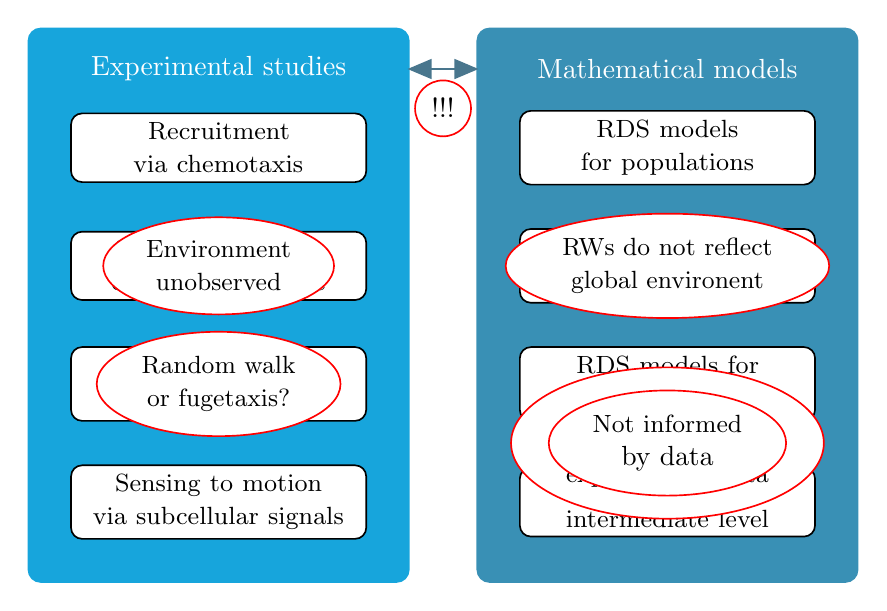
\begin{tikzpicture}[->, >=stealth', auto, semithick, node distance=5em]
	\tikzstyle{block} = [rectangle, draw, fill=white, 
	text width=10em, text centered, rounded corners, minimum height=2em]
	\tikzstyle{line} = [draw, -latex']
	\draw[line width=0.5mm,cyan!90!black,fill=cyan!90!black,text centered, rounded corners] (0,7) rectangle (4.8,0);
	\draw[line width=0.5mm,cyan!70!black,fill=cyan!70!black,text centered, rounded corners] (5.7,7) rectangle (10.5,0);
	\node[align=center,text=white] at (2.4,6.5) (A2){Experimental studies};
	\node[align=center,text=white] at (8.1,6.5) (A2){Mathematical models};
	\draw[>=triangle 45,draw=cyan!50!black,line width=1pt, <->] (4.8,6.5) -- (5.7,6.5);	
	\node[block,align=center] at (2.4,1) (A1){\small{Sensing to motion\\ via subcellular signals}};
	\node[block,align=center] at (2.4,2.5) (A2){\small{Resolution via \\reverse migration}};
	\node[block,align=center] at (2.4,4) (A3){\small \textit{in vivo} microscopy on zebrafish larvae};
	\node[block,align=center] at (2.4,5.5) (A4){\small Recruitment via chemotaxis};
	\node[block,align=center] at (8.1,1) (A5){\small Morphodynamics as intermediate level};
	\node[block,align=center] at (8.1,2.5) (A6){\small RDS models for subcellular species};
	\node[block,align=center] at (8.1,4) (A7){\small Random walk models for single cells};
	\node[block,align=center] at (8.1,5.5) (A8){\small RDS models for populations};
	\invisible<1>{\node[circle,draw=red,fill=white,align=center] at (5.25,6) (A0){!!!};}
	\invisible<1-2>{\node[ellipse,draw=red,fill=white,align=center] at (2.4,4) (A10){\small Environment \\ \small unobserved};}
	\invisible<1-3>{\node[ellipse,draw=red,fill=white,align=center] at (2.4,2.5) (A9){\small Random walk \\\small or fugetaxis?};}
	\invisible<1-4>{\node[ellipse,draw=red,fill=white,align=center] at (8.1,4) (A11){\small RWs do not reflect \\ \small global environent};}
	\invisible<1-5>{\node[ellipse,draw=red,fill=white,align=center] at (8.1,1.75) (A11){\small Models not\\ \small informed by \\ \small experimental data};}
	\invisible<1-6>{\node[ellipse,draw=red,fill=white,align=center] at (8.1,1.75) (A11){\small Not informed \\by data};}
	\end{tikzpicture}
\end{figure}
\end{frame}
\begin{frame}{Multicolumn environments}
Multiple columns can be used anywhere on the slide.
\vspace{1cm}
\begin{columns}
	\begin{column}{5cm}
		\centering
		This is column 1.\\
		With centering.\\
		Width defined in absolute values.
	\end{column}
	\begin{column}{0.45\textwidth}
	This is column 2.\\
	Without centering.\\
	Defined with respect to texwidth.\\
	\end{column}
\end{columns}
\vspace{1cm}
\par Followed by normal text separated by vspace.
\end{frame}
\appendix
\section<presentation>*{\appendixname}
\subsection<presentation>*{References}
\begin{frame}[allowframebreaks]
\printbibliography
\end{frame}
\begin{frame}
\centering
\Huge{Thank you!}\\
\huge{Questions?}
\end{frame}
\end{document}